\documentclass[11pt]{article}
\usepackage[margin=1in]{geometry}
\usepackage{amsmath,amssymb,amsthm,mathtools,bm}
\usepackage{booktabs,array,tabularx,longtable}
\usepackage{graphicx}
\usepackage{microtype}
\usepackage{enumitem}
\usepackage{hyperref}
\usepackage[nameinlink,capitalize]{cleveref}
\usepackage{caption}

\hypersetup{
  colorlinks=true,
  linkcolor=blue,
  citecolor=blue,
  urlcolor=blue,
  pdftitle={Collapsed-Saddle Spectra for Products of Linear Forms: Hermite Leakage and Metric-Dependent Hessian Inertia}
}

\newtheorem{theorem}{Theorem}[section]
\newtheorem{proposition}[theorem]{Proposition}
\newtheorem{corollary}[theorem]{Corollary}
\newtheorem{lemma}[theorem]{Lemma}
\newtheorem{remark}[theorem]{Remark}
\newtheorem{definition}[theorem]{Definition}

\newcommand{\R}{\mathbb{R}}
\newcommand{\one}{\mathbf{1}}
\newcommand{\J}{J}
\newcommand{\perm}{\operatorname{perm}}
\newcommand{\rank}{\operatorname{rank}}
\newcommand{\ind}{\operatorname{index}}
\newcommand{\nul}{\operatorname{nullity}}
\newcommand{\col}{\operatorname{col}}
\newcommand{\Span}{\operatorname{span}}
\newcommand{\tr}{\operatorname{tr}}
\newcommand{\ip}[2]{\left\langle #1,#2\right\rangle}
\newcommand{\norm}[1]{\left\lVert #1\right\rVert}
\newcommand{\F}{\mathrm{F}}
\newcommand{\spec}{\mathrm{spec}}
\newcolumntype{Y}{>{\raggedright\arraybackslash}X}

\title{Collapsed-Saddle Spectra for Products of Linear Forms:\\
Hermite Leakage and Metric-Dependent Hessian Inertia}
\author{}
\date{Preprint draft, version 0.3.1\\26 August 2026}

\begin{document}
\maketitle

\begin{abstract}
We study population least-squares landscapes for a single product of $L$ linear forms under isotropic Gaussian input and derive complete parameter-space Hessian spectra at the fully collapsed repeated-factor critical point.  The analysis compares two coefficient-space metrics induced by the same factorized top-degree coefficient map: Wick normalization isolates the top Gaussian-chaos component and yields permanent covariances, whereas the ordinary product retains all lower-Hermite contractions.

For a rectangular Wick teacher $U\in\R^{d\times L}$ with positive-semidefinite Gram matrix $T=U^\top U$, constant row sum $T\one=\gamma\one$, and rank $r$, the collapsed point has Hessian index $(r-1)(L-1)$, nullity $(d-r+1)(L-1)$, and exactly $d$ positive eigenvalues.  For the ordinary Gaussian product with an orthonormal teacher frame, the corresponding index is $(d-1)(L-1)$ and the nullity is $L-1$.  Hence lower-Hermite contractions convert the ambient sector $\col(U)^\perp\otimes\one^\perp$, of dimension $(d-L)(L-1)$, from Hessian-null to strictly negative curvature.  We call this exact inertia change \emph{Hermite-leakage index inflation}.

We also characterize rank-deficient and zero-row-sum boundaries, prove full parameter-space criticality for the raw collapsed branch, identify the even-order companion branch, give an exact ambient single-direction leakage calculation, and state correlation-dependent asymptotics only within their proved scaling windows.  Automatic-differentiation and exact-moment audits include $d<L$ Wick cases, both even-order raw branches, and correctly embedded quartic escape paths.  Independent formula-level rederivations and computational audits support the central spectra.  A targeted comparison with the closest located primary literature did not identify a direct theorem-level duplicate or short explicit reduction; publication priority remains unresolved.
\end{abstract}

\tableofcontents

\section{Introduction}

Products of linear forms sit at the intersection of several mature theories.  As homogeneous polynomials they form the Chow variety; as parameterized predictors they are multiplicative polynomial networks; under Gaussian population loss their covariances are governed by Wick--Isserlis pairings; and their repeated-factor parameterization creates a singular fiber with a large differential kernel.  These ingredients make the model small enough for exact analysis while retaining a central difficulty of nonlinear learning: the local parameter-space geometry is not determined solely by the represented function.

We analyze the fully collapsed point, where all student factors coincide.  The main question is not merely whether that point is a saddle, but how its complete Hessian inertia depends on three features that are usually studied separately: teacher rank, ambient overparameterization, and the inner product induced by the data distribution.  The answer exposes a sharp distinction between top-chaos and full Gaussian metrics.

Our contributions are:
\begin{enumerate}[label=(\roman*)]
\item \textbf{Rectangular, rank-deficient Wick spectrum.}  For every regular positive-semidefinite teacher Gram matrix $T$ with $T\one=\gamma\one$, we derive the full spectrum in factor coordinates.  If $r=\rank(T)$, the Hessian index is $(r-1)(L-1)$, the nullity is $(d-r+1)(L-1)$, and the positive count is $d$.
\item \textbf{Rectangular raw-Gaussian spectrum.}  For an orthonormal teacher frame, we derive six invariant sectors and their exact eigenvalues for arbitrary order $L$ and ambient dimension $d\ge L$.
\item \textbf{Hermite-leakage index inflation.}  Comparing the same factor parameterization under the Wick and ordinary Gaussian metrics shows that lower-Hermite contractions turn the entire sector $\col(U)^\perp\otimes\one^\perp$ from zero curvature into negative curvature.  The exact Hessian-index increase is $(d-L)(L-1)$.
\item \textbf{Singular boundaries and weak-curvature regimes.}  We identify the rank-one boundary, a zero-row-sum boundary at which the full Hessian vanishes, and correlation regimes in which, after normalization by the teacher squared norm, fixed positive equicorrelation changes the specialization-curvature scale from the exponentially weak orthogonal case to polynomial order in $L$.
\item \textbf{Formula-level novelty assessment.}  We separate what follows from general lift theory from what requires permanent and Gaussian-pairing calculations, and compare the theorem family against the closest tensor, polynomial-network, Chow, and symmetry literature.
\end{enumerate}

The closest prior frameworks are substantial.  Symmetric-tensor work constructs highly symmetric critical points and derives exact or asymptotic Hessian spectra for sums of rank-one powers \cite{arjevani_vinograd}.  Polynomial-network theory treats teacher--student tensor approximation under distribution-induced inner products and gives complete Hessian signatures in the quadratic case \cite{arjevani_polynomial}.  Chow-variety work studies identifiability and the differential geometry of smooth products of linear forms \cite{torrance_vannieuwenhoven,kubjas_geometry}.  General smooth-lift theory explains how first- and second-order derivatives of a parameterization affect critical points \cite{levin_kileel_boumal}.  None of those broad descriptions, by itself, fixes the permanent and Isserlis coefficients at the repeated-factor singular point.  Conversely, our formulas may still be implicit in a more general result that we have not identified.  We therefore report a bounded formula-level comparison and treat this document as a circulation draft, not as a settled priority claim.

\section{Models and notation}

Fix integers $L\geq2$ and $d\geq1$, and let
\[
W=[w_1,\ldots,w_L]\in\R^{d\times L}.
\]
Throughout, $x\sim\mathcal N(0,I_d)$ and $\one\in\R^L$ denotes the all-ones vector.  We write $J=\one\one^\top$.

\subsection{Wick product model}

Let
\[
G_W(x)=:\!\prod_{a=1}^{L}w_a^\top x\!:
\]
denote the order-$L$ multivariate Wick product.  The Gaussian-chaos covariance identity gives
\begin{equation}
\mathbb E[G_W(x)G_U(x)]=\perm(W^\top U).
\label{eq:wick-permanent}
\end{equation}
Thus, for a teacher $U\in\R^{d\times L}$, the population loss is
\begin{equation}
\mathcal L_U(W)
=\frac12\left[
\perm(W^\top W)-2\perm(W^\top U)+\perm(U^\top U)
\right].
\label{eq:wick-loss}
\end{equation}

\subsection{Ordinary Gaussian product model}

The raw product is
\[
F_W(x)=\prod_{a=1}^{L}w_a^\top x.
\]
For an orthonormal teacher frame $U=[u_1,\ldots,u_L]$, $U^\top U=I_L$, set
\[
\tau_U(x)=\prod_{i=1}^{L}u_i^\top x.
\]
The population loss is
\begin{equation}
\mathcal R_U(W)=\frac12\mathbb E[(F_W(x)-\tau_U(x))^2].
\label{eq:raw-loss}
\end{equation}
Unlike \eqref{eq:wick-loss}, the student norm in \eqref{eq:raw-loss} contains all pairings of $2L$ Gaussian factors, including lower-chaos self-contractions.

Both objectives use the same factorized homogeneous degree-$L$ coefficient map (equivalently, the same Chow-cone parameterization of the top-degree coefficient tensor), but they equip its image with different population inner products.  The Wick-ordered and ordinary student functions are therefore not pointwise identical polynomial expressions.  For an orthonormal teacher frame, however, the teacher Wick product and the ordinary teacher product coincide because cross-contractions among distinct teacher coordinates vanish.

\subsection{Inertia convention}
For a symmetric Hessian $H$, we write
\[
\ind(H)=n_-(H),\qquad \nul(H)=n_0(H),
\]
where eigenvalues are counted with algebraic multiplicity.

\section{Lift-level decomposition of factor-space curvature}
\label{sec:lift-decomposition}

The distinction between parameterization effects and metric-specific effects is made explicit by a standard second-order chain rule.

\begin{proposition}[Gauss--Newton and residual curvature]
\label{prop:chain-rule-curvature}
Let $\mathcal H$ be a real Hilbert space, let $\Phi:\R^{d\times L}\to\mathcal H$ be twice differentiable, and define
\[
\mathcal E(W)=\frac12\norm{\Phi(W)-\tau}_{\mathcal H}^2.
\]
Then, for every perturbation $H$,
\begin{equation}
D^2\mathcal E(W)[H,H]
=
\norm{D\Phi(W)[H]}_{\mathcal H}^2
+
\ip{\Phi(W)-\tau}{D^2\Phi(W)[H,H]}_{\mathcal H}.
\label{eq:chain-rule-curvature}
\end{equation}
In particular, on $\ker D\Phi(W)$ the Hessian is determined entirely by the residual-curvature term.
\end{proposition}

\begin{proof}
Differentiate $D\mathcal E(W)[H]=\ip{\Phi(W)-\tau}{D\Phi(W)[H]}_{\mathcal H}$ once more in the same direction.
\end{proof}

Here $\Phi$ denotes the formal homogeneous top-degree coefficient map, represented by its ordinary polynomial.  In the Wick model, the same coefficient tensor is realized in the $L$th Gaussian chaos by Wick ordering; the pointwise Wick differential is the Wick-ordered counterpart of the display below and has the same kernel $H\one=0$.

For the formal top-degree product map
\[
\Phi(W)(x)=\prod_{a=1}^{L}w_a^\top x
\]
at a repeated-factor point $W=c\,m\one^\top$ with $c\ne0$ and $m\ne0$,
\begin{equation}
D\Phi(W)[H](x)
=c^{L-1}(m^\top x)^{L-1}(H\one)^\top x.
\label{eq:product-differential}
\end{equation}
Hence
\begin{equation}
\ker D\Phi(W)=\{H:H\one=0\},
\qquad
\dim\ker D\Phi(W)=d(L-1).
\label{eq:product-kernel}
\end{equation}
The first-order kernel contains both genuine infinitesimal gauge directions and directions that change the represented polynomial only at second order.  General lift theory predicts that the latter may acquire residual curvature, but it does not determine its sign or multiplicity without the particular target and function-space metric.  The Wick/raw comparison below computes that residual term exactly: on the ambient specialization sector it vanishes under the top-chaos metric and is strictly negative under the full Gaussian metric.

\begin{remark}[Scope of the general reduction]
Equation~\eqref{eq:chain-rule-curvature} explains the mechanism class but does not imply the spectra in \cref{thm:wick-rectangular,thm:raw-spectrum}.  Obtaining those formulas still requires: (i) permanent derivatives at a constant rank-one matrix; (ii) exact Gaussian cross-moments with the teacher; and (iii) a simultaneous invariant-sector decomposition that tracks teacher-span, ambient, collective, specialization, radial, and gauge directions.
\end{remark}

\section{Permanent calculus at a constant rank-one matrix}

The following elementary identity drives the Wick analysis.

\begin{lemma}[Permanent derivatives]
\label{lem:permanent-derivatives}
Let $p(A)=\perm(A)$ for $A\in\R^{L\times L}$, and let $A_0=\alpha J$.  For $E,F\in\R^{L\times L}$, define
\[
s(E)=\one^\top E\one,\qquad r(E)=E\one,\qquad c(E)=E^\top\one.
\]
Then
\begin{equation}
Dp(A_0)[E]=(L-1)!\alpha^{L-1}s(E),
\label{eq:perm-first}
\end{equation}
and
\begin{align}
D^2p(A_0)[E,F]
=(L-2)!\alpha^{L-2}\bigl(&s(E)s(F)-r(E)^\top r(F)\nonumber\\
&-c(E)^\top c(F)+\ip{E}{F}_{\F}\bigr).
\label{eq:perm-second}
\end{align}
\end{lemma}

\begin{proof}
For the first derivative, fix the differentiated entry.  The remaining $L-1$ rows and columns can be matched in $(L-1)!$ ways, and every remaining product equals $\alpha^{L-1}$.  Summing over the differentiated entry yields \eqref{eq:perm-first}.

For the second derivative, two differentiated entries contribute only when they occupy distinct rows and distinct columns.  Summing over all ordered pairs and excluding same-row and same-column pairs by inclusion--exclusion gives
\[
s(E)s(F)-r(E)^\top r(F)-c(E)^\top c(F)+\ip{E}{F}_{\F}.
\]
The remaining $L-2$ entries contribute $(L-2)!\alpha^{L-2}$.
\end{proof}

\section{Rectangular and rank-deficient Wick teachers}

\subsection{Regular positive-semidefinite teachers}

Let
\begin{equation}
T=U^\top U\succeq0,
\qquad T\one=\gamma\one,
\qquad \gamma>0,
\label{eq:regular-psd}
\end{equation}
and set $r=\rank(T)=\rank(U)$.  Since the eigenvector $\one$ has positive eigenvalue $\gamma$, the restriction of $T$ to $\one^\perp$ has exactly $r-1$ positive eigenvalues.  Denote them by
\[
\mu_1,\ldots,\mu_{r-1}>0.
\]
Define the collapsed point and scale
\begin{equation}
W_\star=\frac1L UJ,
\qquad
b_L(T)=(L-2)!\left(\frac{\gamma}{L}\right)^{L-2}.
\label{eq:wick-collapsed-scale}
\end{equation}

\begin{theorem}[Rectangular regular-PSD Wick spectrum]
\label{thm:wick-rectangular}
Under \eqref{eq:regular-psd}, $W_\star$ is a critical point of \eqref{eq:wick-loss}.  Its critical value is
\begin{equation}
\mathcal L_U(W_\star)
=\frac12\left[
\perm(T)-L!\left(\frac{\gamma}{L}\right)^L
\right].
\end{equation}
The full Hessian spectrum in the $dL$-dimensional parameter space is
\begin{center}
\begin{tabular}{@{}lll@{}}
\toprule
Sector & Eigenvalue & Multiplicity\\
\midrule
Radial & $L(L-1)\gamma b_L(T)$ & $1$\\
Gauge & $0$ & $L-1$\\
Teacher collective $i$ & $(L-1)(\gamma+\mu_i)b_L(T)$ & one for each $i$\\
Teacher specialization $i$ & $-\mu_i b_L(T)$ & $L-1$ for each $i$\\
Ambient collective & $(L-1)\gamma b_L(T)$ & $d-r$\\
Ambient null & $0$ & $(d-r)(L-1)$\\
\bottomrule
\end{tabular}
\end{center}
Consequently,
\begin{equation}
\boxed{\ind(W_\star)=(r-1)(L-1)},
\qquad
\boxed{\nul(W_\star)=(d-r+1)(L-1)},
\label{eq:wick-inertia}
\end{equation}
and the number of positive eigenvalues is exactly $d$.
\end{theorem}

\begin{proof}
Let $e=\one/\sqrt L$.  Since $\norm{Ue}^2=\gamma$, define
\[
p_0=\frac{Ue}{\sqrt\gamma}.
\]
Choose an orthonormal eigenbasis $q_1,\ldots,q_{L-1}$ of $\one^\perp$ such that $Tq_i=\mu_iq_i$ for $i\leq r-1$, while $Tq_i=0$ for $i\geq r$.  For $i\leq r-1$, let
\[
p_i=\frac{Uq_i}{\sqrt{\mu_i}}.
\]
Then $p_0,p_1,\ldots,p_{r-1}$ is an orthonormal basis of $\col(U)$.  Complete it with an orthonormal basis $n_1,\ldots,n_{d-r}$ of $\col(U)^\perp$.

At $W_\star$,
\[
W_\star^\top W_\star=W_\star^\top U=\frac{\gamma}{L}J.
\]
The first derivative of the student norm cancels the first derivative of the cross term, by \cref{lem:permanent-derivatives}; hence $W_\star$ is critical.

For perturbations $H,K$, let
\[
E_H=W_\star^\top H+H^\top W_\star,
\qquad F_H=H^\top U.
\]
Differentiating \eqref{eq:wick-loss} twice gives
\begin{align}
D^2\mathcal L_U(W_\star)[H,K]
={}&\frac12D^2p(A)[E_H,E_K]
+\frac12Dp(A)[H^\top K+K^\top H]\nonumber\\
&-D^2p(A)[F_H,F_K],
\label{eq:wick-bilinear-hessian}
\end{align}
where $A=(\gamma/L)J$.

Now use the orthonormal tensor-product basis
\[
p_0e^\top,
\quad p_0q_j^\top,
\quad p_ie^\top,
\quad p_iq_j^\top,
\quad n_ae^\top,
\quad n_aq_j^\top.
\]
Substitution into \eqref{eq:wick-bilinear-hessian} and \eqref{eq:perm-second} shows that distinct basis elements are Hessian-orthogonal and yields, respectively,
\[
L(L-1)\gamma b_L,
\quad0,
\quad(L-1)(\gamma+\mu_i)b_L,
\quad-\mu_i b_L,
\quad(L-1)\gamma b_L,
\quad0.
\]
The multiplicities sum to
\[
1+(L-1)+(r-1)+(r-1)(L-1)+(d-r)+(d-r)(L-1)=dL.
\]
The inertia follows because $\gamma>0$ and all listed $\mu_i$ are positive.
\end{proof}

\begin{corollary}[Orthonormal rectangular teacher]
\label{cor:wick-orthonormal}
If $U^\top U=I_L$ and $d\geq L$, then
\[
\ind(W_\star)=(L-1)^2,
\qquad
\nul(W_\star)=(d-L+1)(L-1),
\qquad n_+(W_\star)=d.
\]
The ambient subspace $\col(U)^\perp\otimes\one^\perp$ is Hessian-null.
\end{corollary}

\subsection{Singular boundaries}

\begin{corollary}[Rank-one boundary]
\label{cor:rank-one-boundary}
If $r=1$, then $T=(\gamma/L)J$, all teacher columns coincide, and $W_\star=U$ is an exact global minimizer.  Its Hessian is positive semidefinite with
\[
\ind(W_\star)=0,
\qquad
\nul(W_\star)=d(L-1),
\qquad n_+(W_\star)=d.
\]
\end{corollary}

\begin{proposition}[Zero-row-sum boundary]
\label{prop:gamma-zero}
Suppose $T\succeq0$, $T\one=0$, and $L\geq3$.  Then $U\one=0$ and the collapsed point is $W_\star=0$.  For every $H\in\R^{d\times L}$ and scalar $t$,
\begin{equation}
\mathcal L_U(tH)-\mathcal L_U(0)
=-t^L\perm(H^\top U)+\frac12t^{2L}\perm(H^\top H).
\label{eq:gamma-zero-exact}
\end{equation}
In particular, both the gradient and Hessian at zero vanish identically.
\end{proposition}

\begin{proof}
Positive semidefiniteness and $T\one=0$ imply
\[
\norm{U\one}^2=\one^\top T\one=0.
\]
The identity \eqref{eq:gamma-zero-exact} follows from degree-$L$ homogeneity of the permanent.  For $L\geq3$, its Taylor expansion has no linear or quadratic term.
\end{proof}

\section{Rectangular raw Gaussian products}

Assume henceforth that $d\geq L$ and $U^\top U=I_L$.  Set
\[
m=U\one,\qquad P=UU^\top,
\]
so that $\norm{m}^2=L$.  Along the collapsed ray $W=c\,m\one^\top$, the student is $c^L(m^\top x)^L$.  Gaussian moments give
\[
\mathbb E[(m^\top x)^{2L}]=(2L-1)!!L^L,
\qquad
\mathbb E[\tau_U(x)(m^\top x)^L]=L!.
\]
Let $c_L>0$ denote the positive real root of
\begin{equation}
\boxed{
c_L^L=\frac{L!}{L^L(2L-1)!!}
=\frac{2^L(L!)^2}{L^L(2L)!}
}.
\label{eq:raw-c}
\end{equation}
Define
\[
W_\star^{\rm raw}=c_Lm\one^\top
\]
and
\begin{equation}
k_L=(L-2)!c_L^{L-2}.
\label{eq:raw-k}
\end{equation}

\begin{proposition}[Full raw criticality and the even-order companion]
\label{prop:raw-criticality}
The point $W_\star^{\rm raw}$ is a critical point of \eqref{eq:raw-loss} in the full $dL$-dimensional parameter space.  If $L$ is even, then $-W_\star^{\rm raw}$ is a second collapsed critical representative of the same predictor and has the same Hessian spectrum.
\end{proposition}

\begin{proof}
Write $S=m^\top x$.  At $W=c_Lm\one^\top$, the gradient with respect to any column $w_a$ is
\begin{align}
\nabla_{w_a}\mathcal R_U(W)
={}&c_L^{2L-1}\mathbb E[S^{2L-1}x]
-c_L^{L-1}\mathbb E[\tau_U S^{L-1}x].
\label{eq:raw-full-gradient}
\end{align}
Gaussian integration by parts gives
\[
\mathbb E[S^{2L-1}x]=(2L-1)!!L^{L-1}m.
\]
Rotating to the orthonormal teacher coordinates and counting the surviving monomials gives
\[
\mathbb E[\tau_U S^{L-1}x]=(L-1)!m.
\]
Consequently,
\[
\nabla_{w_a}\mathcal R_U(W)
=c_L^{L-1}\left[
 c_L^L(2L-1)!!L^{L-1}-(L-1)!
\right]m=0
\]
by \eqref{eq:raw-c}.  This holds for every column, proving full parameter-space criticality.

If $L$ is even, replacing $c_L$ by $-c_L$ leaves the predictor unchanged because $(-c_L)^L=c_L^L$.  The same gradient cancellation applies, and all Hessian coefficients below depend on the branch only through $c_L^{L-2}$, which is also unchanged for even $L$.
\end{proof}

\subsection{Gaussian moment identities}

For a perturbation $H=[h_1,\ldots,h_L]$, define
\[
r=H\one,\qquad q=H^\top m,\qquad s=m^\top H\one.
\]
Let $S=m^\top x$, $Y=r^\top x$, and $y_a=h_a^\top x$.  The first two parameter derivatives of the student are
\[
F'=c_L^{L-1}S^{L-1}Y,
\qquad
F''=c_L^{L-2}S^{L-2}\left(Y^2-\sum_a y_a^2\right).
\]
Two moment identities are useful.  For arbitrary $v,w\in\R^d$,
\begin{align}
\mathbb E[S^{2L-2}(v^\top x)(w^\top x)]
=(2L-3)!!L^{L-2}\bigl(&L v^\top w\nonumber\\
&+2(L-1)(m^\top v)(m^\top w)\bigr),
\label{eq:student-moment}
\end{align}
and
\begin{equation}
\mathbb E[\tau_U(x)S^{L-2}(v^\top x)(w^\top x)]
=(L-2)!\left[(m^\top v)(m^\top w)-v^\top Pw\right].
\label{eq:teacher-cross-moment}
\end{equation}
Equation \eqref{eq:teacher-cross-moment} follows after rotating to the teacher coordinates: the relevant $L\times L$ moment matrix is $(L-2)!(J-I)$, while all ambient contributions vanish.

\begin{theorem}[Raw rectangular Hessian quadratic form]
\label{thm:raw-quadratic}
At $W_\star^{\rm raw}$,
\begin{align}
\frac{D^2\mathcal R_U(W_\star^{\rm raw})[H,H]}{k_L}
={}&\left[\frac{4(L-1)^2}{L(2L-1)}-1\right]s^2
+\frac{2(L-1)}{2L-1}\norm{r}^2+\norm{Pr}^2\nonumber\\
&+\frac{3L-2}{L(2L-1)}\norm{q}^2
-\frac{L-1}{2L-1}\norm{H}_{\F}^2-\norm{PH}_{\F}^2.
\label{eq:raw-qform}
\end{align}
\end{theorem}

\begin{proof}
Use
\[
D^2\mathcal R_U[H,H]=\mathbb E[(F')^2+(F-\tau_U)F''].
\]
Apply \eqref{eq:student-moment} to $Y^2$ and every $y_a^2$, apply \eqref{eq:teacher-cross-moment} to the teacher cross term, and simplify with the critical relation
\[
c_L^L L^L(2L-1)!!=L!.
\]
Collecting the coefficients of $s^2$, $\norm r^2$, $\norm{Pr}^2$, $\norm q^2$, $\norm H_\F^2$, and $\norm{PH}_\F^2$ yields \eqref{eq:raw-qform}.
\end{proof}

\begin{theorem}[Raw rectangular spectrum]
\label{thm:raw-spectrum}
By \cref{prop:raw-criticality}, $W_\star^{\rm raw}$ is critical.  Its full Hessian spectrum is
\begin{center}
\begin{tabular}{@{}lll@{}}
\toprule
Sector & Eigenvalue & Multiplicity\\
\midrule
Radial & $L(L-1)k_L$ & $1$\\
Gauge & $0$ & $L-1$\\
Teacher collective & $2(L-1)k_L$ & $L-1$\\
Teacher specialization & $-\dfrac{3L-2}{2L-1}k_L$ & $(L-1)^2$\\
Ambient collective & $(L-1)k_L$ & $d-L$\\
Ambient specialization & $-\dfrac{L-1}{2L-1}k_L$ & $(d-L)(L-1)$\\
\bottomrule
\end{tabular}
\end{center}
Consequently,
\begin{equation}
\boxed{\ind(W_\star^{\rm raw})=(d-1)(L-1)},
\qquad
\boxed{\nul(W_\star^{\rm raw})=L-1},
\label{eq:raw-inertia}
\end{equation}
and the number of positive eigenvalues is $d$.
\end{theorem}

\begin{proof}
Let $e=\one/\sqrt L$ and $p_0=m/\sqrt L$.  Choose an orthonormal basis $q_1,\ldots,q_{L-1}$ of $\one^\perp$ and set $p_i=Uq_i$.  Complete $p_0,p_1,\ldots,p_{L-1}$ to an orthonormal basis of $\R^d$ with $n_1,\ldots,n_{d-L}$.

Evaluate \eqref{eq:raw-qform} on the orthonormal tensor-product basis
\[
p_0e^\top,
\quad p_0q_j^\top,
\quad p_ie^\top,
\quad p_iq_j^\top,
\quad n_ae^\top,
\quad n_aq_j^\top.
\]
The six eigenvalues obtained are, in the same order,
\[
L(L-1)k_L,
\quad0,
\quad2(L-1)k_L,
\quad-\frac{3L-2}{2L-1}k_L,
\quad(L-1)k_L,
\quad-\frac{L-1}{2L-1}k_L.
\]
The cross terms vanish because the basis simultaneously diagonalizes the projectors onto $\Span\{m\}$, $\col(U)\cap m^\perp$, and $\col(U)^\perp$, as well as the right factors $\Span\{\one\}$ and $\one^\perp$.  Counting multiplicities gives \eqref{eq:raw-inertia}.
\end{proof}

\section{Hermite-leakage index inflation}

The Wick and raw objectives share the same factor coordinates and the same top-degree coefficient map, but they induce different inner products on the resulting polynomial coefficient space.  Their rectangular spectra therefore admit a direct comparison.

\begin{corollary}[Hermite-leakage index inflation]
\label{thm:hermite-leakage}
Let $U\in\R^{d\times L}$ have orthonormal columns, with $d\geq L$.  At their respective collapsed critical points,
\begin{align}
\ind_{\rm Wick}&=(L-1)^2,
&\nul_{\rm Wick}&=(d-L+1)(L-1),\\
\ind_{\rm raw}&=(d-1)(L-1),
&\nul_{\rm raw}&=L-1.
\end{align}
Hence
\begin{equation}
\boxed{
\ind_{\rm raw}-\ind_{\rm Wick}=(d-L)(L-1)
}.
\label{eq:index-inflation}
\end{equation}
The additional negative eigenspace is exactly
\[
\col(U)^\perp\otimes\one^\perp.
\]
It is Hessian-null in the Wick model and has raw eigenvalue
\begin{equation}
-\frac{L-1}{2L-1}k_L
\label{eq:ambient-raw-negative}
\end{equation}
with multiplicity $(d-L)(L-1)$.
\end{corollary}

\begin{proof}
The inertia identities follow from \cref{cor:wick-orthonormal,thm:raw-spectrum}.  To expose the mechanism on the additional sector, choose unit vectors
\[
n\perp\col(U),\qquad q\perp\one,
\]
and set $H=nq^\top$.  Then $H\one=0$, $H^\top m=0$, and $PH=0$.  Thus the first derivative of the raw student vanishes:
\[
F'=c_L^{L-1}S^{L-1}(H\one)^\top x=0.
\]
Moreover,
\[
F''=-c_L^{L-2}S^{L-2}(n^\top x)^2,
\]
because $H\one=0$ and $\sum_a q_a^2=1$.  The teacher cross moment is zero because $n\perp\col(U)$, whereas the raw student residual retains the self-contraction of the two ambient factors and contributes
\begin{align*}
D^2\mathcal R_U(W_\star^{\rm raw})[H,H]
&=-c_L^{2L-2}\mathbb E[S^{2L-2}]\mathbb E[(n^\top x)^2]\\
&=-c_L^{2L-2}(2L-3)!!L^{L-1}\\
&=-\frac{L-1}{2L-1}k_L.
\end{align*}
In the Wick model, ordering removes this lower-chaos self-contraction, and \cref{cor:wick-orthonormal} gives zero curvature on the same sector.  Its dimension is
\[
\dim\col(U)^\perp\,\dim\one^\perp=(d-L)(L-1),
\]
which proves \eqref{eq:index-inflation} and identifies the additional negative eigenspace.
\end{proof}

\begin{remark}[Parameterization and residual curvature]
At a fully repeated factor, the differential of the product map depends only on $H\one$, so every column-sum-zero perturbation is first-order invisible.  Gauge directions remain in the exact parameter fiber.  Other first-order invisible directions can acquire second-order curvature through the residual term
\[
\ip{F_W-\tau}{D^2F_W[H,H]}.
\]
The Wick metric cancels this contribution on ambient specialization directions, while lower-Hermite self-contractions in the raw metric make it strictly negative.
\end{remark}

\begin{figure}[t]
\centering
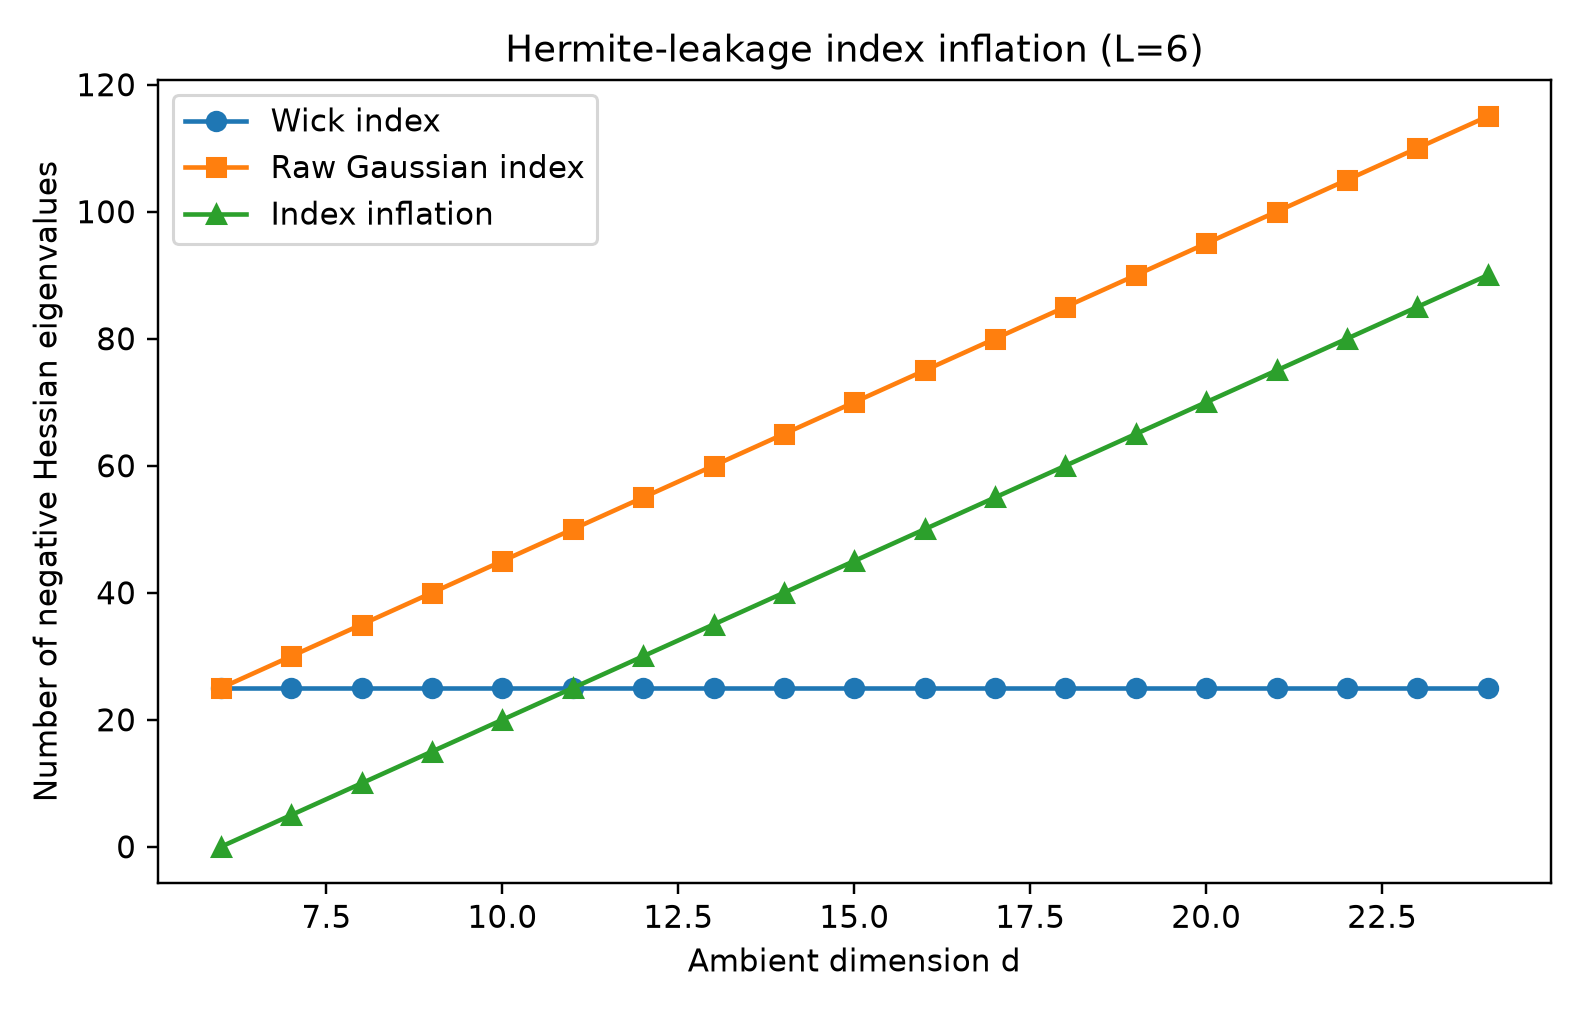
\includegraphics[width=0.78\textwidth]{../plots/hermite_leakage_index_inflation.png}
\caption{For fixed order $L=6$, the Wick index is independent of the ambient dimension, whereas the raw Gaussian index grows linearly with $d$.  The difference is exactly $(d-L)(L-1)$.}
\label{fig:index-inflation}
\end{figure}

\section{Weak-curvature scaling and singular transitions}

\subsection{Orthogonal teachers}
For the Wick model,
\[
a_L=\frac{(L-2)!}{L^{L-2}}
\sim\sqrt{2\pi L}\,e^{-L}.
\]
Thus the number of negative directions grows quadratically in $L$ while each specialization curvature becomes exponentially weak.

For the raw model, the teacher-span specialization curvature obeys
\[
\left|\lambda_{\rm teacher,spec}^{\rm raw}\right|
\sim6\sqrt2\,\pi L(2e)^{-L},
\]
while the ambient specialization curvature obeys
\[
\left|\lambda_{\rm ambient,spec}^{\rm raw}\right|
\sim2\sqrt2\,\pi L(2e)^{-L}.
\]
The raw metric therefore creates more strict descent directions but makes their scale even smaller.

\subsection{Equicorrelated Wick teachers}
Let
\[
T_\rho=(1-\rho)I+\rho J,
\qquad -\frac1{L-1}<\rho<1.
\]
Then
\[
\gamma=1+(L-1)\rho,
\qquad \mu=1-\rho,
\]
and every specialization eigenvalue is
\begin{equation}
-(1-\rho)(L-2)!\left(\frac{1+(L-1)\rho}{L}\right)^{L-2}.
\label{eq:equicorr-spec}
\end{equation}
As $\rho\uparrow1$, these $(L-1)^2$ negative eigenvalues approach zero.  At $\rho=1$, the Gram rank drops to one, \cref{cor:rank-one-boundary} applies, and the index jumps from $(L-1)^2$ to zero.

After normalizing by the teacher squared norm $\perm(T_\rho)$, positive correlation changes the asymptotic weak-curvature class.  The exact normalized specialization curvature can be written without an unproved regime extrapolation.

\begin{proposition}[Exact equicorrelation normalization and a restricted crossover]
\label{prop:equicorr-normalized}
For $0<\rho<1$, let
\[
x=\frac{1-\rho}{\rho},
\qquad
E_L(x)=\sum_{j=0}^{L}\frac{x^j}{j!}.
\]
Then
\begin{equation}
\frac{|\lambda_{\rm spec}(T_\rho)|}{\perm(T_\rho)}
=
\frac{x(x+1)}{L(L-1)}
\frac{(1+x/L)^{L-2}}{E_L(x)}.
\label{eq:equicorr-exact-normalized}
\end{equation}
For every fixed $\rho\in(0,1)$,
\begin{equation}
\frac{|\lambda_{\rm spec}(T_\rho)|}{\perm(T_\rho)}
\sim
\frac{1-\rho}{\rho^2L(L-1)}.
\label{eq:equicorr-fixed-rho}
\end{equation}
More generally, suppose $\rho_L\sqrt L\to t\in(0,\infty)$.  Then
\begin{equation}
\frac{|\lambda_{\rm spec}(T_{\rho_L})|}{\perm(T_{\rho_L})}
\sim
\frac{e^{-1/(2t^2)}}{t^2L}.
\label{eq:equicorr-sqrt-window}
\end{equation}
No claim is made here that $\rho_L\sqrt L$ alone classifies all regimes with $\rho_L\to0$ outside this window.
\end{proposition}

\begin{proof}
Since $T_\rho=\rho(J+xI)$,
\[
\perm(T_\rho)=\rho^LL!E_L(x).
\]
Also $1+(L-1)\rho=\rho(L+x)$.  Substitution into \eqref{eq:equicorr-spec} gives \eqref{eq:equicorr-exact-normalized}.  For fixed $x$, $E_L(x)\to e^x$ and $(1+x/L)^{L-2}\to e^x$, proving \eqref{eq:equicorr-fixed-rho}.

The assumption $\rho_L\sqrt L\to t\in(0,\infty)$ implies $x_L/\sqrt L\to t^{-1}$, hence $x_L=O(\sqrt L)$ and $x_L=o(L)$.  Therefore
\[
\frac{E_L(x_L)}{e^{x_L}}
=\Pr\{\operatorname{Poisson}(x_L)\le L\}
\longrightarrow 1,
\]
for example by a standard Poisson upper-tail bound.  Moreover,
\[
(L-2)\log(1+x_L/L)-x_L
=-\frac{x_L^2}{2L}+o(1).
\]
Applying these relations to \eqref{eq:equicorr-exact-normalized} yields \eqref{eq:equicorr-sqrt-window}.
\end{proof}

\begin{figure}[t]
\centering
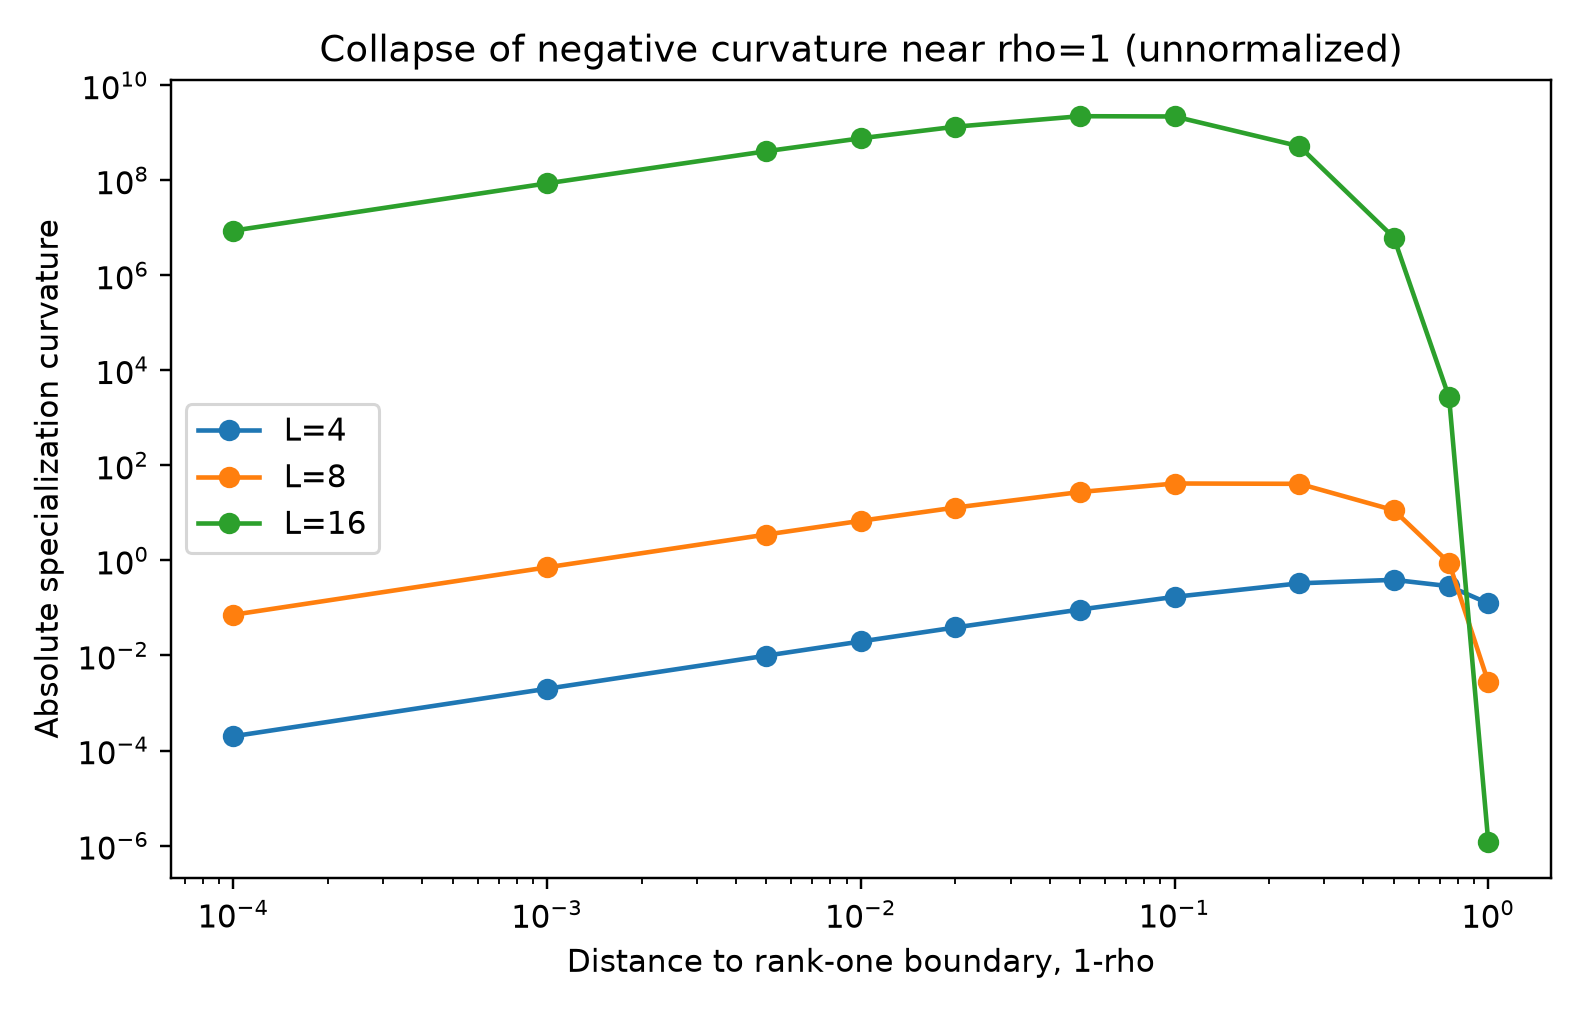
\includegraphics[width=0.78\textwidth]{../plots/equicorrelation_rank_one_boundary.png}
\caption{Unnormalized specialization curvature as $\rho\uparrow1$.  It vanishes at the rank-one boundary $\rho=1$; the index remains $(L-1)^2$ for every full-rank point and drops only at the singular boundary.}
\label{fig:rho-boundary}
\end{figure}

\section{Exact restricted escape and its limitation}

\begin{proposition}[Correctly embedded quartic contrast path]
\label{prop:quartic-path}
For an orthonormal Wick teacher $U\in\R^{d\times L}$, choose distinct indices $i\ne j$ and $p\ne q$, and define
\[
K=\frac12(e_i-e_j)(e_p-e_q)^\top.
\]
Then $K\one=K^\top\one=0$, $\norm K_\F=1$, and along the rectangularly embedded path
\[
W(t)=U\left(\frac1LJ+tK\right)
\]
one has
\begin{equation}
\mathcal L_U(W(t))-\mathcal L_U(W(0))
=-\frac{a_L}{2}t^2+\frac{a_L}{4}t^4,
\qquad
 a_L=\frac{(L-2)!}{L^{L-2}}.
\label{eq:quartic-path}
\end{equation}
\end{proposition}

\begin{proof}
Write $e=\one/\sqrt L$ and $K=uv^\top$, where
\[
u=\frac{e_i-e_j}{\sqrt2},
\qquad
v=\frac{e_p-e_q}{\sqrt2}.
\]
Then $u,v\perp e$ and $\norm u=\norm v=1$.  With
\[
A(t)=ee^\top+tuv^\top,
\qquad W(t)=UA(t),
\]
orthonormality of $U$ gives
\[
W(t)^\top U=A(t)^\top,
\qquad
W(t)^\top W(t)=ee^\top+t^2vv^\top.
\]
At $A_0=ee^\top=J/L$, the first permanent derivatives in the two contrast directions vanish.  By \cref{lem:permanent-derivatives},
\[
\perm(A(t)^\top)=\perm(A_0)+\frac{a_L}{2}t^2,
\qquad
\perm(A(t)^\top A(t))=\perm(A_0)+\frac{a_L}{2}t^4.
\]
There are no higher-order terms because each contrast has only two nonzero rows and two nonzero columns.  Substitution into \eqref{eq:wick-loss} proves \eqref{eq:quartic-path}.
\end{proof}

The projected gradient flow on this path is
\[
\dot t=a_Lt(1-t^2),
\]
so the exact projected time from $0<\varepsilon<r<1$ is
\begin{equation}
T_{\varepsilon\to r}^{\rm proj}
=\frac1{a_L}\left[
\log\frac r\varepsilon
-\frac12\log\frac{1-r^2}{1-\varepsilon^2}
\right].
\end{equation}
After an orthogonal coordinate reduction one may equivalently take $d=L$, $U=I_L$, and write $W(t)=J/L+tK$.  The affine line is generally not invariant under the full ambient gradient flow, so this is a constrained theorem rather than a full nonlinear escape theorem.  Recent work on saddle-structured dynamics in nonlinear networks illustrates why obtaining full invariant reductions and escape laws is substantially stronger than local Hessian analysis \cite{rawal_deweese}.

\clearpage
\section{Relation to existing frameworks and formula-level duplication audit}
\label{sec:novelty-audit}

\subsection{Closest frameworks}

\begingroup
\small
\setlength{\LTleft}{0pt}
\setlength{\LTright}{0pt}
\begin{longtable}{@{}>{\raggedright\arraybackslash}p{0.19\textwidth}>{\raggedright\arraybackslash}p{0.23\textwidth}>{\raggedright\arraybackslash}p{0.52\textwidth}@{}}
\toprule
Source family & Closest overlap & What is not supplied directly \\
\midrule
\endfirsthead
\toprule
Source family & Closest overlap & What is not supplied directly \\
\midrule
\endhead
\midrule
\multicolumn{3}{r}{\footnotesize Continued on next page}\\
\endfoot
\bottomrule
\endlastfoot
Symmetric tensor decomposition \cite{arjevani_vinograd} & Symmetry-adapted critical points; exact/asymptotic Hessian spectra; index calculations & The model is a sum of symmetric rank-one powers rather than one Chow product; the repeated-factor Wick/raw formulas and ambient index conversion are not stated. \\
Shallow polynomial networks \cite{arjevani_polynomial} & Teacher--student tensor approximation under data-induced inner products; complete quadratic Gaussian landscape & The complete signature theorem is for quadratic activations; it does not give arbitrary-order products of distinct linear factors or the six-sector raw spectrum. \\
Chow geometry \cite{torrance_vannieuwenhoven,kubjas_geometry} & Products of linear forms as an algebraic variety; identifiability, smooth loci, and geometric invariants & The collapsed repeated-factor point has a singular parameter fiber; the cited results do not state the full factor-coordinate population-loss Hessian there. \\
Linear convolutional networks \cite{kohn_geometry_lcn,kohn_function_space_lcn} & Polynomial factorization models, function-space geometry, repeated filters, and parameterization criticality; Theorem~2.11 of \cite{kohn_function_space_lcn} characterizes criticality through common factors & These results do not evaluate the Wick/raw Gaussian population Hessian or its signed six-sector spectrum at the repeated-factor point. \\
Polynomial convolutional and neuromanifold geometry \cite{shahverdi_polyconv,shahverdi_razor} & Regularity, singular strata, dimensions, degrees, and generic critical-point counts; Proposition~4.11 of \cite{shahverdi_polyconv} concerns counts rather than types & The local factor-coordinate Hessian coefficients and inertia at the present singular collapsed fiber remain model-specific. \\
Degenerate metrics on algebraic varieties \cite{marchetti_degenerate} & Projection and ramification methods for critical points under degenerate quadratic objectives & The framework concerns critical-point geometry and counting, not the explicit signed Hessian spectrum under the two Gaussian-chaos metrics used here. \\
Deep monomial singular learning \cite{kohn_deep_monomial} & Theorem-level links between parameterization criticality and inactive or redundant subnetworks at high activation degree & The result is Jacobian/criticality-level and does not provide the permanent/Isserlis Hessian coefficients or rectangular multiplicities. \\
Smooth parametrizations \cite{levin_kileel_boumal,trager_pure} & General first/second-order chain rules; spurious criticality and parameterization-induced curvature & The framework yields \eqref{eq:chain-rule-curvature}, but not the permanent/Isserlis coefficients, invariant multiplicities, or metric-dependent inertia. \\
Inner-product-dependent tensor distance \cite{kozhasov_inner_products} & Algebraic complexity of critical points changes with tensor inner product & It counts generic critical points through ED degree rather than resolving the local signed spectrum at a fixed singular factorization. \\
Permanent/product optimization \cite{yuan_parrilo} & Exact connection between products of linear forms and positive-semidefinite permanents & A different optimization objective; no teacher--student collapsed Hessian or Wick/raw comparison. \\
Approximate symmetries \cite{kuhn_rosenow} & Exact symmetry zero modes and their lifting under model perturbations & The present null-to-negative conversion is an exact population formula caused by lower-Hermite contractions, with a specified eigenspace and multiplicity. \\
\end{longtable}
\endgroup

\subsection{Direct-duplication criterion}

For this audit, a prior result counts as a \emph{direct formula-level duplicate} only if it supplies, either explicitly or by an immediate substitution, all of the following:
\begin{enumerate}[label=(D\arabic*)]
\item the factor parameterization by one product of $L$ linear forms, rather than a sum of powers or a generic tensor rank model;
\item the fully repeated-factor collapsed point, including its singular parameter fiber;
\item the Wick/top-chaos or ordinary Gaussian population inner product with the corresponding teacher term; and
\item the signed factor-coordinate spectrum with multiplicities in rectangular or rank-deficient regimes, sufficient to recover \eqref{eq:wick-inertia}, \eqref{eq:raw-inertia}, or \eqref{eq:index-inflation} without a new model-specific Hessian calculation.
\end{enumerate}

The targeted search covered exact theorem names and formulas, products-of-linear-forms/Chow geometry, symmetric-tensor Hessian spectra, polynomial-network teacher metrics, smooth-lift Hessian formulas, inner-product-dependent tensor distance, permanent optimization, and symmetry-induced zero modes.  No located source met all four criteria.  In particular:
\begin{itemize}
\item symmetry methods explain why a small number of sectors should occur, but the representation and coefficients differ;
\item smooth-lift theory gives the decomposition \eqref{eq:chain-rule-curvature}, but leaves the residual bilinear form model-dependent;
\item smooth-locus Chow geometry does not directly cover the repeated-factor singular parameter point; and
\item quadratic polynomial-network landscape results do not specialize to arbitrary product order.
\end{itemize}

\subsection{Formula-level novelty assessment}

Independent formula-level rederivations and computational audits reproduced the core spectra, including $d<L$, even-order branch, and embedded-path checks.  A targeted comparison with the primary sources listed above did not locate a direct theorem-level duplicate or short explicit reduction.  The appropriate conclusion remains deliberately asymmetric:
\begin{quote}
The theorem family survives a targeted formula-level duplication search and is not a one-line quotation of the closest located results.  It remains strongly embedded in mature frameworks and may be an unstated corollary of a broader theorem.  The search was bounded rather than exhaustive, publication priority remains unresolved, and accountable human peer review has not yet been established.
\end{quote}

This status is stronger than ``an interesting calculation'' but weaker than ``a proven new theorem in the literature.''  The present draft makes no breakthrough claim and does not infer novelty from the absence of a keyword match.

\section{Computer-assisted verification}

The analytic formulas were checked independently using automatic differentiation and exact finite Gaussian moment calculations.  The verification code is included with this note.

\begin{center}
\begin{tabular}{@{}lrr@{}}
\toprule
Audit & Cells & Maximum absolute error\\
\midrule
Rectangular/rank-deficient Wick spectra (including $d<L$) & 28 & $5.1\times10^{-13}$\\
Rank-one Wick boundary & 8 & $2.05\times10^{-12}$\\
Zero-row-sum exact identity & 60 & $4.46\times10^{-13}$\\
Rectangular raw spectra & 9 & $2.66\times10^{-15}$\\
Raw quadratic-form directions & 72 & $8.88\times10^{-15}$\\
Even-order raw positive/negative branches & 6 & $<2\times10^{-15}$\\
Embedded quartic paths & 6 & $<10^{-15}$\\
Ambient Hermite-leakage unit directions & 5 & $<10^{-14}$\\
Analytic inertia counts & 242 & $0$ mismatches\\
\bottomrule
\end{tabular}
\end{center}

The Wick permanent is evaluated by a differentiable Ryser formula.  The raw student norm is evaluated independently by summing perfect Gaussian pairings.  Full automatic-differentiation Hessians are diagonalized for small orders and random embeddings.  Version 0.3.1 includes the $d<L$ Wick cases, both even-order raw branches, the rectangularly embedded quartic path, and direct unit-direction checks of the ambient Hermite-leakage coefficient.  The code is diagnostic support, not a substitute for the proofs.

\section{Limitations, circulation status, and next step}

The results are local, population-level statements for a highly structured model.  They do not establish global convergence, a full ambient nonlinear escape theorem, an SGD law, or dominance of the same mechanism in practical neural networks.  The raw theorem assumes an orthonormal teacher frame; a general raw regular-teacher formula remains open in this development.  The computational audit verifies finite instances but is not a substitute for the analytic proofs.

The novelty assessment is also bounded.  It uses targeted searches, theorem-level comparison against the closest located primary sources, and independent formula-level rederivations and computational audits.  It is not a systematic review of every tensor, invariant-theory, singularity, and algebraic-statistics result.  Accordingly, this version is \emph{ready for ordinary expert circulation, while human peer review and publication priority remain unresolved}.

The targeted comparison did not locate an immediate reduction of the rectangular Wick spectrum, the arbitrary-order raw six-sector spectrum, or the exact ambient null-to-negative conversion in the primary sources examined.  The next legitimate step is accountable human expert circulation and, if appropriate after that review, submission as a compact theorem note while maintaining a conservative priority claim.  A direct reduction supplied later should still demote the affected claims to worked corollaries.  Further theorem-family expansion, architecture design, and broad neural benchmarking remain outside the scope of this revision.

\appendix

\section{Sector table for a representative rectangular model}

For $L=6$ and $d=10$, the exact sector values and multiplicities are visualized in \cref{fig:sector-spectrum}.  The plot emphasizes that the raw ambient sector has nonzero positive and negative curvatures, while the Wick ambient specialization sector is null.

\begin{figure}[h]
\centering
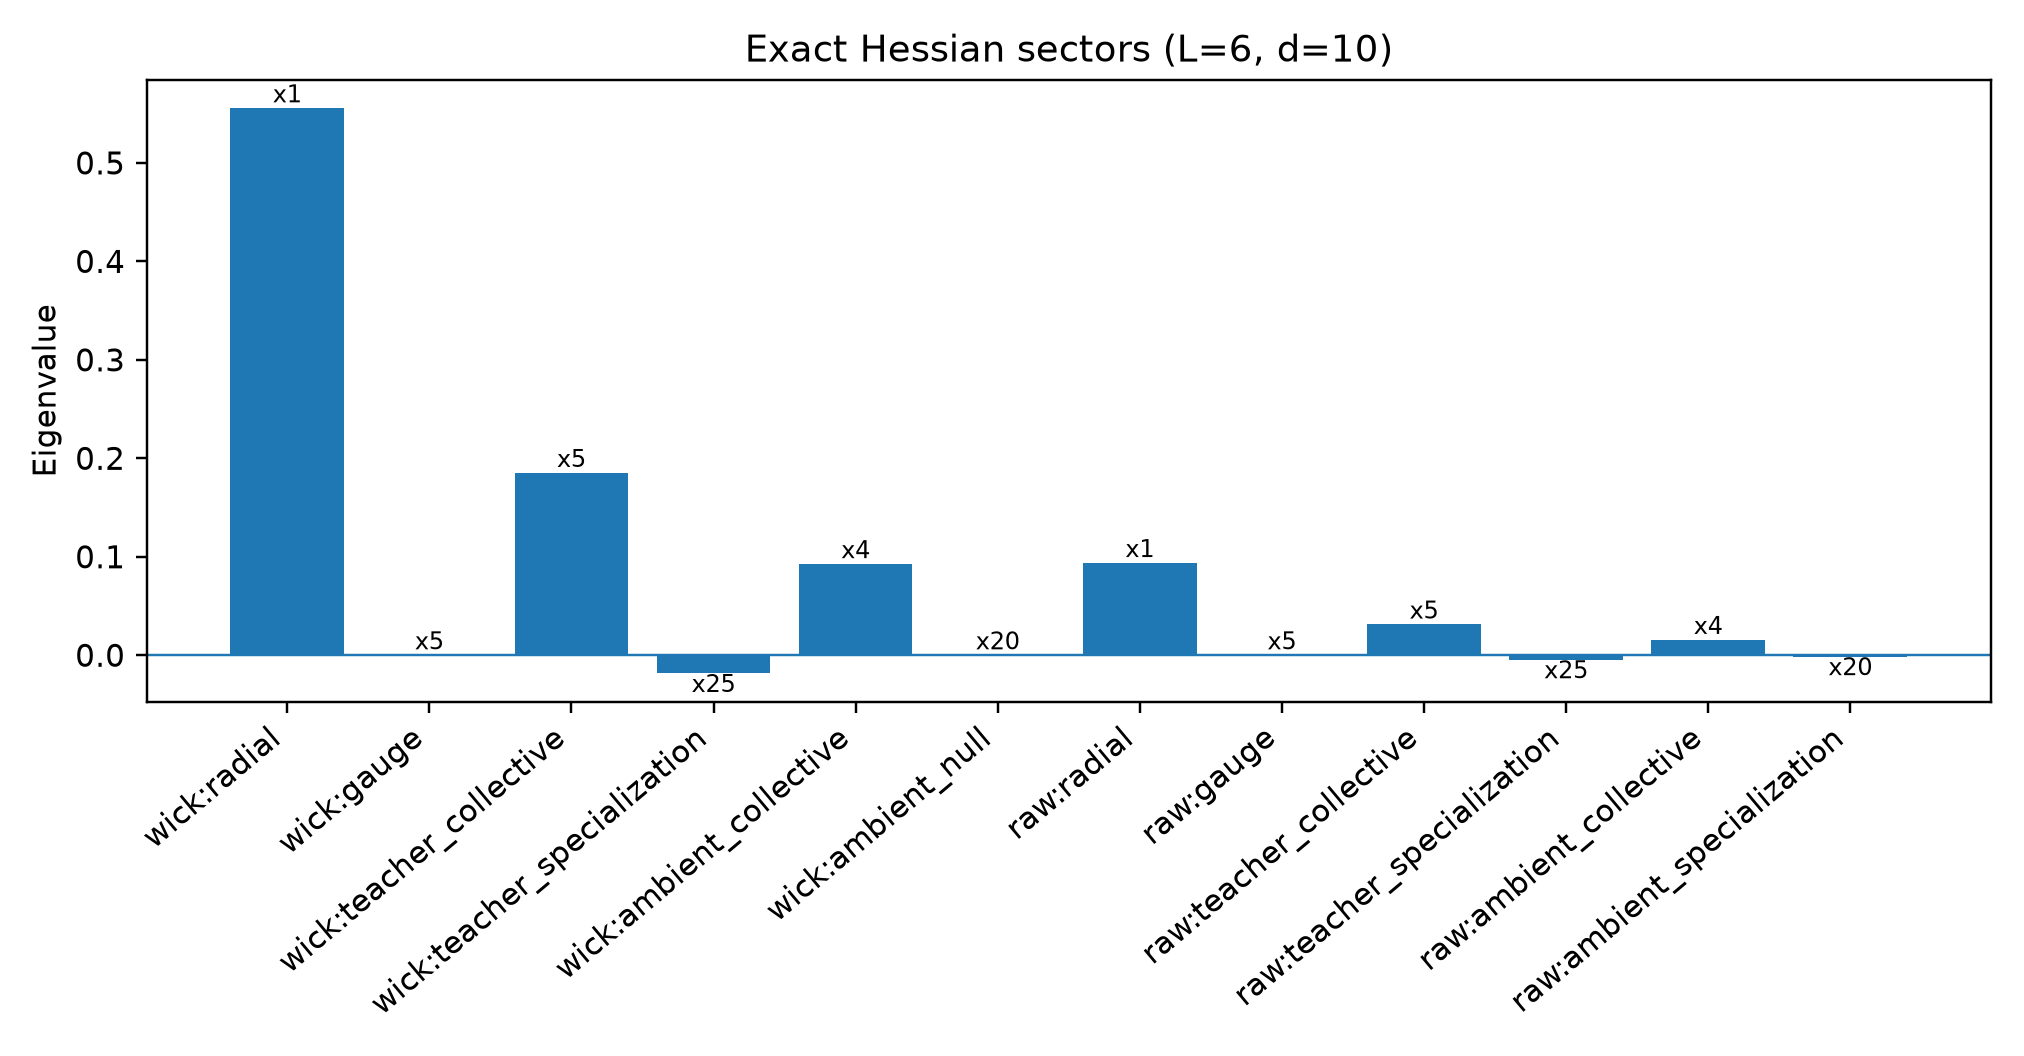
\includegraphics[width=0.96\textwidth]{../plots/sector_spectrum_comparison.png}
\caption{Sector eigenvalues and multiplicities for $L=6$, $d=10$.  Values are unnormalized; annotations show multiplicities.}
\label{fig:sector-spectrum}
\end{figure}

\section{Rank dependence of Wick inertia}

At fixed $L$ and $d$, \cref{eq:wick-inertia} gives a linear exchange between index and nullity as the teacher Gram rank changes, while the positive count remains $d$.

\begin{figure}[h]
\centering
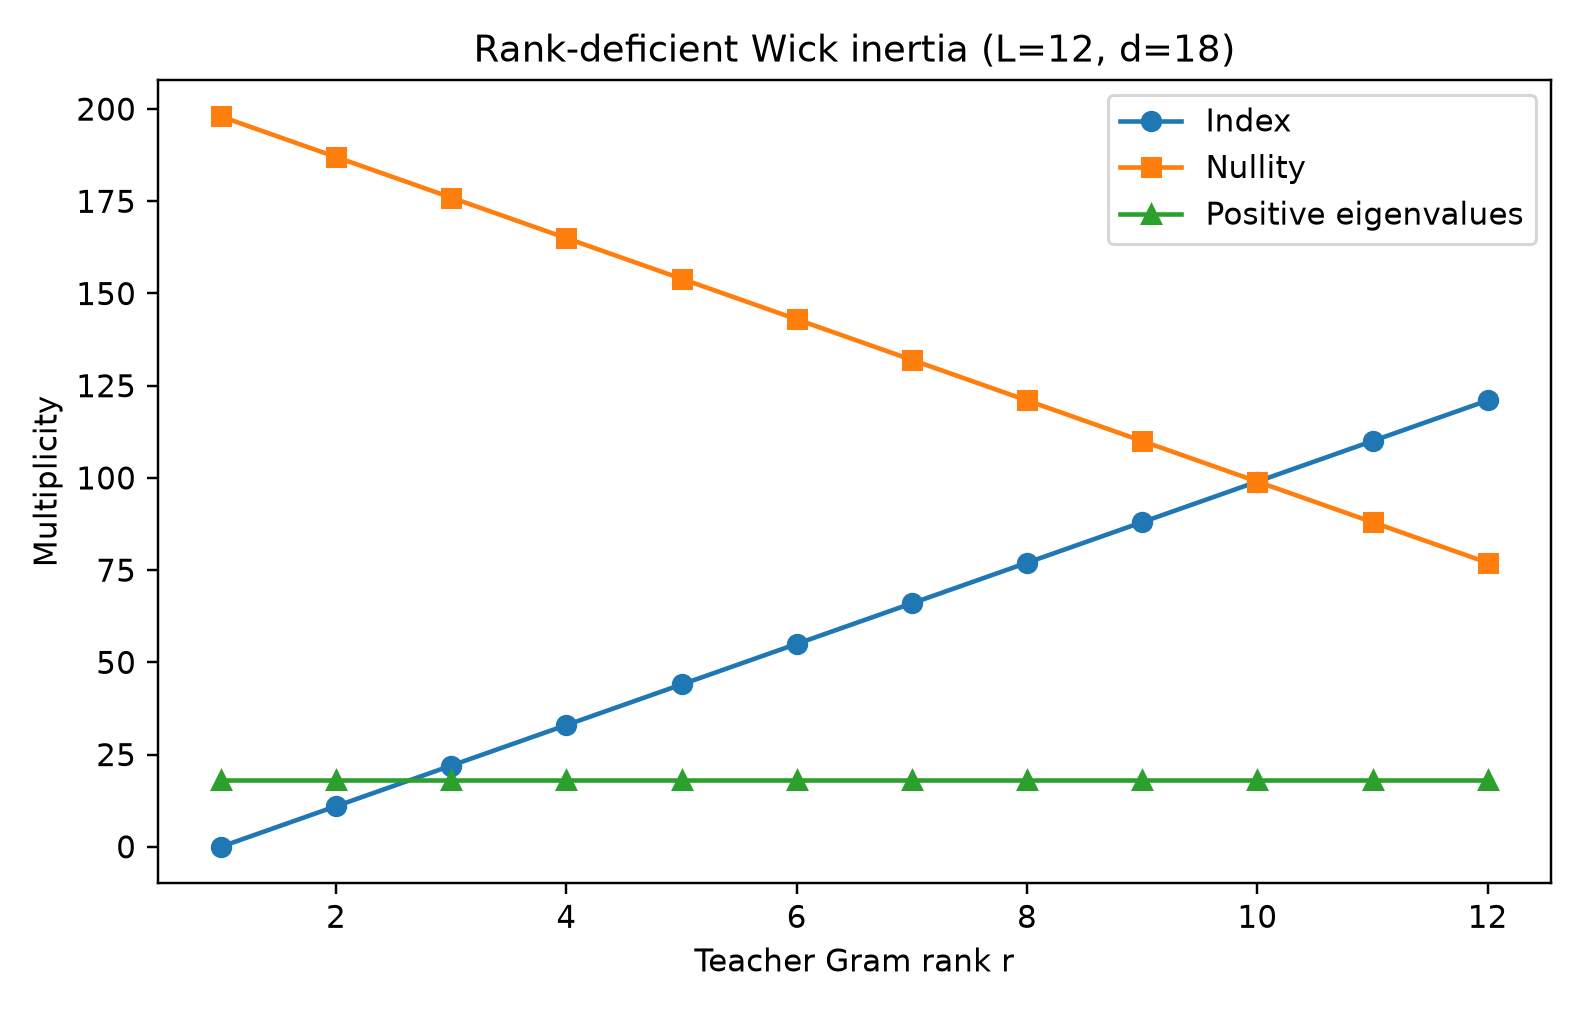
\includegraphics[width=0.82\textwidth]{../plots/wick_rank_deficiency_bifurcation.png}
\caption{Exact inertia as a function of teacher Gram rank for $L=12$, $d=18$.}
\end{figure}

\begin{thebibliography}{99}

\bibitem{arjevani_vinograd}
Y.~Arjevani and G.~Vinograd.
\newblock Symmetry \& critical points for symmetric tensor decomposition problems.
\newblock \emph{arXiv:2306.07886}, version 5, 2025.

\bibitem{arjevani_polynomial}
Y.~Arjevani, J.~Bruna, J.~Kileel, E.~Polak, and M.~Trager.
\newblock Geometry and optimization of shallow polynomial networks.
\newblock \emph{SIAM Journal on Applied Algebra and Geometry}, 10(2):174--209, 2026.
\newblock doi:10.1137/25M1732994.

\bibitem{torrance_vannieuwenhoven}
D.~A. Torrance and N.~Vannieuwenhoven.
\newblock Almost all subgeneric third-order Chow decompositions are identifiable.
\newblock \emph{Annali di Matematica Pura ed Applicata}, 201:2891--2905, 2022.
\newblock doi:10.1007/s10231-022-01224-8.

\bibitem{kubjas_geometry}
K.~Kubjas, J.~Li, and M.~Wiesmann.
\newblock Geometry of polynomial neural networks.
\newblock \emph{Algebraic Statistics}, 15(2):295--328, 2024.
\newblock doi:10.2140/astat.2024.15.295.

\bibitem{levin_kileel_boumal}
E.~Levin, J.~Kileel, and N.~Boumal.
\newblock The effect of smooth parametrizations on nonconvex optimization landscapes.
\newblock \emph{Mathematical Programming}, 209:63--111, 2025.
\newblock doi:10.1007/s10107-024-02058-3.

\bibitem{trager_pure}
M.~Trager, K.~Kohn, and J.~Bruna.
\newblock Pure and spurious critical points: A geometric study of linear networks.
\newblock \emph{arXiv:1910.01671}, 2019.

\bibitem{kozhasov_inner_products}
K.~Kozhasov, A.~Muniz, Y.~Qi, and L.~Sodomaco.
\newblock On the minimal algebraic complexity of the rank-one approximation problem for general inner products.
\newblock Accepted in \emph{Mathematics of Computation}, 2025.
\newblock doi:10.1090/mcom/4176; arXiv:2309.15105v3.

\bibitem{yuan_parrilo}
C.~Yuan and P.~A. Parrilo.
\newblock Maximizing products of linear forms, and the permanent of positive semidefinite matrices.
\newblock \emph{arXiv:2002.04149}, 2020.

\bibitem{kuhn_rosenow}
M.~K\"uhn and B.~Rosenow.
\newblock Explaining near-zero Hessian eigenvalues through approximate symmetries in neural networks.
\newblock \emph{arXiv:2607.07845}, 2026.

\bibitem{rawal_deweese}
D.~Rawal and M.~R. DeWeese.
\newblock A theory of saddle escape in deep nonlinear networks.
\newblock \emph{arXiv:2605.01288}, version 2, 2026.

\bibitem{kohn_geometry_lcn}
K.~Kohn, T.~Merkh, G.~Mont\'ufar, and M.~Trager.
\newblock Geometry of linear convolutional networks.
\newblock \emph{SIAM Journal on Applied Algebra and Geometry}, 6(3):368--406, 2022.
\newblock doi:10.1137/21M1441183.

\bibitem{kohn_function_space_lcn}
K.~Kohn, G.~Mont\'ufar, V.~Shahverdi, and M.~Trager.
\newblock Function space and critical points of linear convolutional networks.
\newblock \emph{SIAM Journal on Applied Algebra and Geometry}, 8(2):333--362, 2024.
\newblock doi:10.1137/23M1565504; arXiv:2304.05752.

\bibitem{shahverdi_polyconv}
V.~Shahverdi, G.~L. Marchetti, and K.~Kohn.
\newblock On the geometry and optimization of polynomial convolutional networks.
\newblock In \emph{Proceedings of the 28th International Conference on Artificial Intelligence and Statistics}, volume 258 of \emph{Proceedings of Machine Learning Research}, pages 604--612, 2025.
\newblock arXiv:2410.00722.

\bibitem{shahverdi_razor}
V.~Shahverdi, G.~L. Marchetti, and K.~Kohn.
\newblock Learning on a razor's edge: Identifiability and singularity of polynomial neural networks.
\newblock In \emph{International Conference on Learning Representations}, 2026.
\newblock arXiv:2505.11846v3.

\bibitem{marchetti_degenerate}
G.~L. Marchetti, E.~Connelly, P.~Breiding, and K.~Kohn.
\newblock Critical points of degenerate metrics on algebraic varieties: A tale of overparametrization.
\newblock \emph{arXiv:2512.21029}, 2025.

\bibitem{kohn_deep_monomial}
K.~Kohn, G.~L. Marchetti, F.~Shabir, V.~Shahverdi, and W.~Wang.
\newblock Singular learning and Occam's razor in deep monomial networks.
\newblock \emph{arXiv:2606.28464}, 2026.

\bibitem{isserlis}
L.~Isserlis.
\newblock On a formula for the product-moment coefficient of any order of a normal frequency distribution in any number of variables.
\newblock \emph{Biometrika}, 12(1/2):134--139, 1918.

\bibitem{janson}
S.~Janson.
\newblock \emph{Gaussian Hilbert Spaces}.
\newblock Cambridge University Press, 1997.

\end{thebibliography}

\end{document}
